\doublespacing
\chapter{Design} \label{chap:design}

%\version{v1.10.2015}


\doublespacing
\section{Data Flow Diagram}
The data flow diagram of our application is given below in Figure \ref{fig:DFD}. It explains that we have three components and each component interact with each other by sending request while doing their task fulfill.
\begin{figure}[!h]
    \centering
    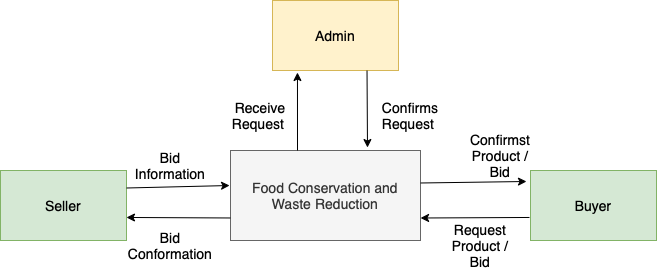
\includegraphics[width=15cm, height=15cm, keepaspectratio ]{Data Flow Diagram.drawio-2.png}
    \caption{Data Flow Diagram}
    
    \label{fig:DFD}
\end{figure}
\newpage
\section{Sequence Diagram}
This is the sequence diagram of our web application and it is the  representation of the system as whole, how buyer and seller will login to our system. The Buyer is going to create a bid. The request will transfer to the bid manager then it is going to come back with result. Same will happen to Bidding, The bid manager sends the request to bidding and then bidding will update the status of the product that is on bid. The sequence diagram of our web application is listed below in Figure \ref{fig:SD} : \\
\begin{figure}[!h]
    \centering
    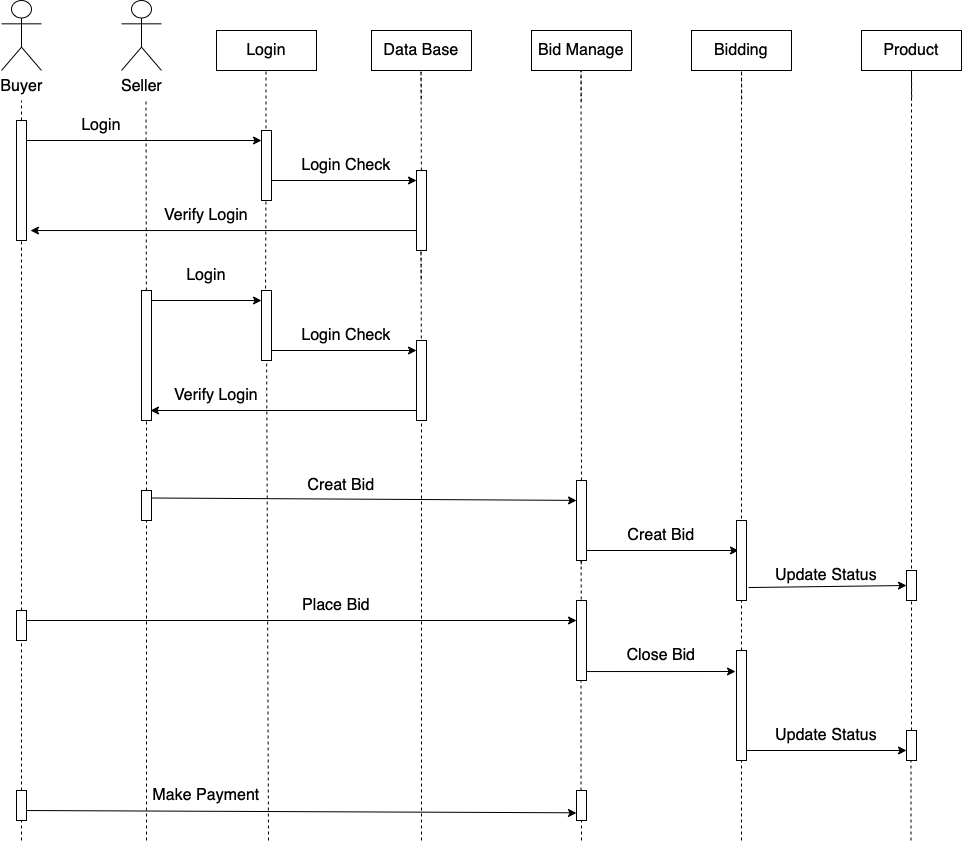
\includegraphics[width=15cm, height=15cm, keepaspectratio ]{Updated Final Sequence Diagram.drawio.png}
    \caption{Sequence Diagram of system}
    \label{fig:SD}
\end{figure}
\section{Use Case Diagram}
The use case diagram of our web application explains how user is going to interact in our application. The all the functionalities that user can perform in our web application is represented in usecase figure \ref{fig:UCD1}, \ref{fig:UCD2}. The users for our web application will be buyer, seller and admin and their use cases are following.

\subsection{For Users}
The use case diagram for Buyers and Sellers is shown in following Figure \ref{fig:UCD1}. The buyer can sign up and sign in to the system. Buyer can search for the product, apply for bid and browse items in the system. The seller can sign up and sign in to the system. Seller can manage item, place items for bidding. \\
\begin{figure}[!h]
    \centering
    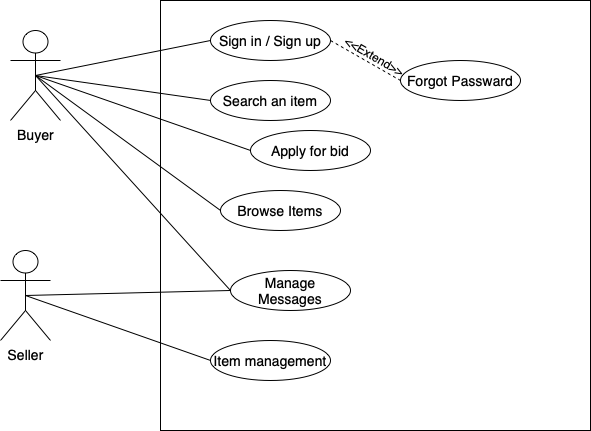
\includegraphics[width=15cm, height=15cm, keepaspectratio ]{Usecase Diagram Diagram.drawio.png}
    \caption{Use Case Diagram For Users}
    \label{fig:UCD1}
\end{figure}
\newpage
\subsection{For Admin}
The use case diagram for Admin is shown in following Figure   \ref{fig:UCD2}. The admin can login to the system. Admin can manage items like modify data about items, access data of items. Admin can manage users in the system.\\
\begin{figure}[!h]
    \centering
    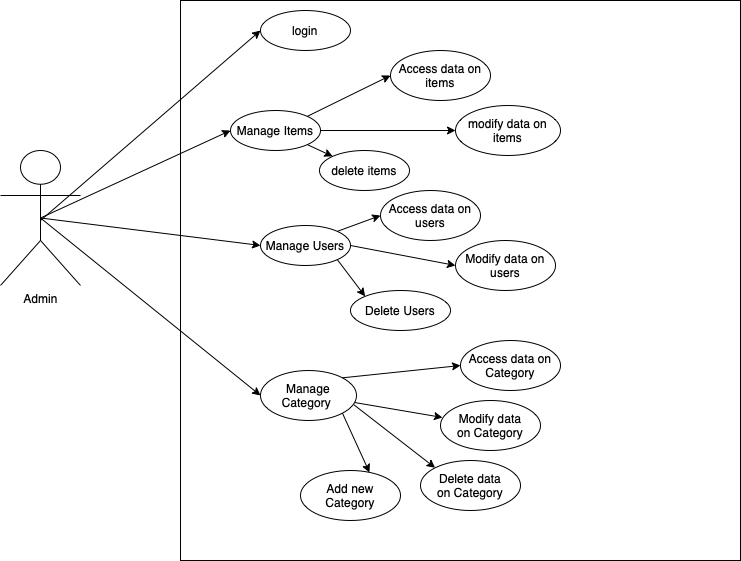
\includegraphics[width=15cm, height=15cm, keepaspectratio ]{Usecase Admin.drawio.png}
    \caption{Use Case Diagram For Admin}
    \label{fig:UCD2}
\end{figure}

\section{Activity Diagram}
The activity diagram of our web application representation all the activities throughout our web application. In these diagrams you will be able to see clear overview of our web application.

\subsection{For Sign Up/Login In}
The activity diagram for Sign up and Login is in following Figure \ref{fig:AD1}. The users enters the login page. If user is registered then user will be simply logged in. The new user will register first and then enters in the web application to perform bidding. \\
\begin{figure}[!h]
    \centering
    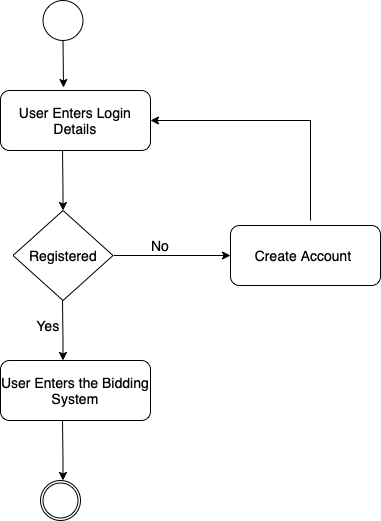
\includegraphics[width=15cm, height=15cm, keepaspectratio ]{Activity Diagram.drawio.png}
    \caption{Activity Diagram For Sign Up/Login}
    \label{fig:AD1}
\end{figure}

\subsection{For Bidding}
The activity diagram for complete process of bidding is shown in following Figure \ref{fig:AD2}. The user will first search for the item. If the item is available then user will check if the bidding is open on the searched item. The user will then apply bid on the item. If user won the bid, user will be notified. Then user will proceed to the payment method.
\begin{figure}[!h]
    \centering
    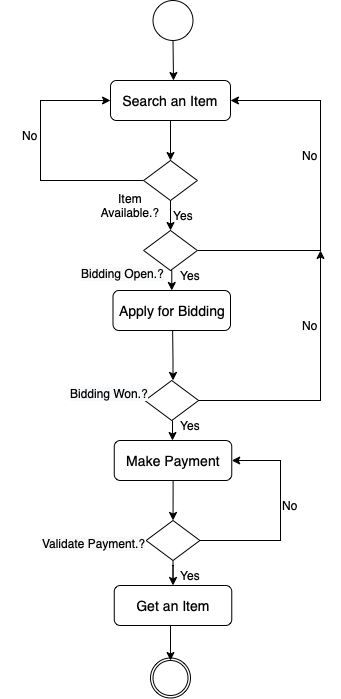
\includegraphics[width=15cm, height=15cm, keepaspectratio ]{Activity Diagram Process.drawio.png}
    \caption{Activity Diagram For Bidding}
    \label{fig:AD2}
\end{figure}
\newpage
\section{ER Diagram}
\doublespacing
\textbf{Entities}
 \\
\textbf{User:} This entity captures information about the buyer or seller who signed up on our web application portal.\\
\textbf{Administrator:} The entity captures the information about all the individuals who are responsible for the functioning of web application.\\
\textbf{Product:} This entity captures the information about all the products which are available for the Bidding.\\
\textbf{Bidding:} This entity captures the information about any product which is already on a bid.\\
\textbf {Feedback:} This entity captures the information about reaction/feedback of any buyer or seller about any product on bidding.\\
\textbf{Bid:} This entity captures the information about the bid any buyer has put for a product i.e. the price a buyer is willing to pay in an bidding.\\
\textbf{Payment Method:} This entity captures the information about chosen payment method for any sold product by a buyer or accepted payment methods by seller for any product.
The following is ER Diagram shown in Figure \ref{fig:ER} :\\
\begin{figure}[!h]
    \centering
    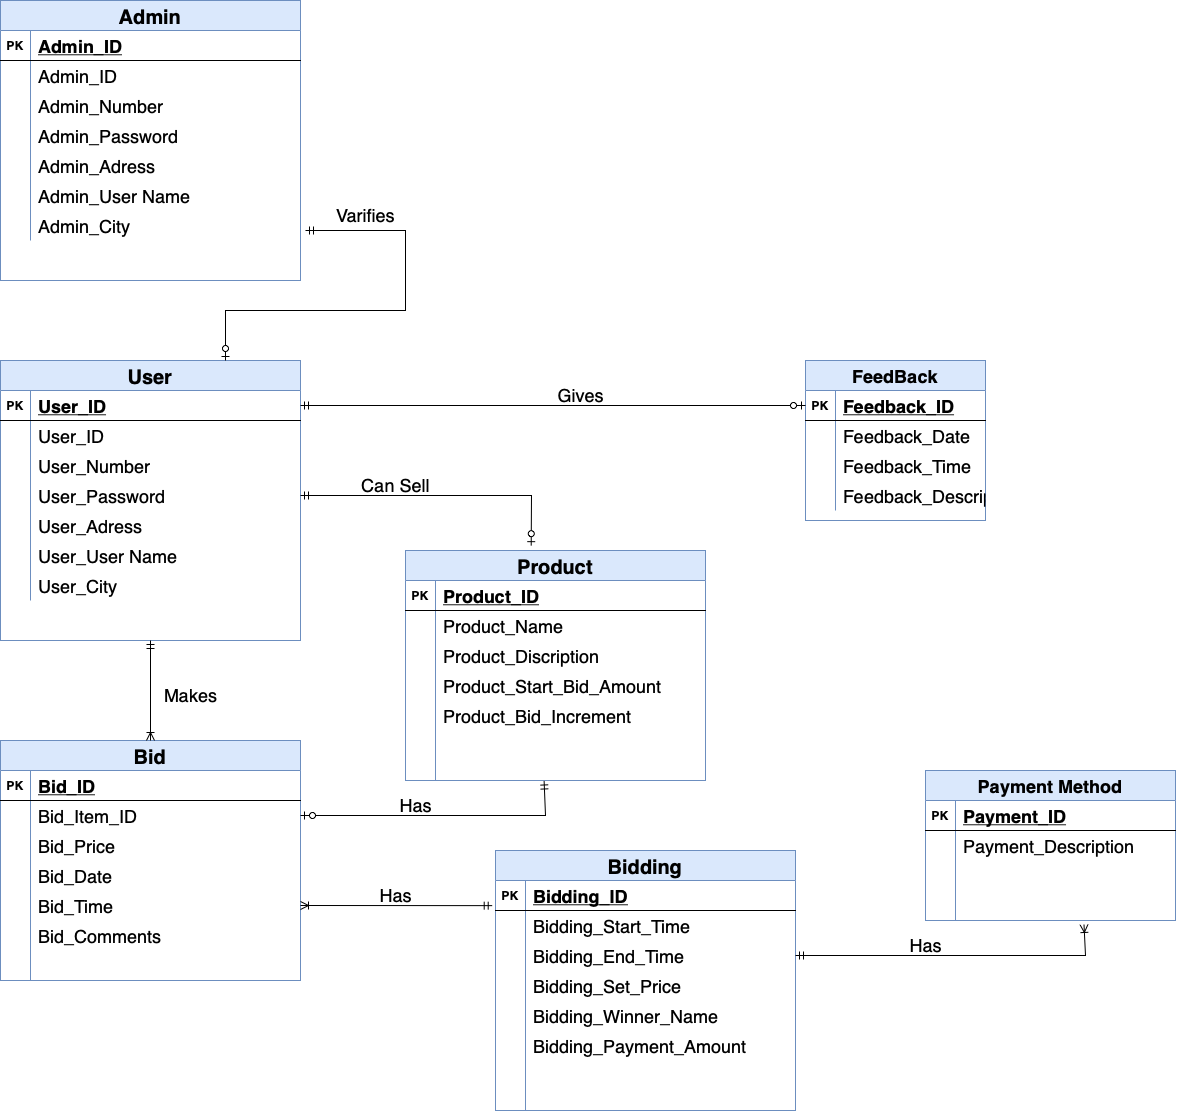
\includegraphics[width=15cm, height=15cm, keepaspectratio ]{Final ER Diagram.drawio.png}
    \caption{ER Diagram}
    \label{fig:ER}
\end{figure}\\
\newpage
\section{Deployment Diagram}
The Deployment Diagram of our web application is shown in following Figure \ref{DD}. The deployment diagram shows the relation between hardware and software in the system and the processing distribution. The components of the web application runs on across the devices shows physical arrangement of nodes in distributed system.  \\\\

\begin{figure}[!h]
    \centering
    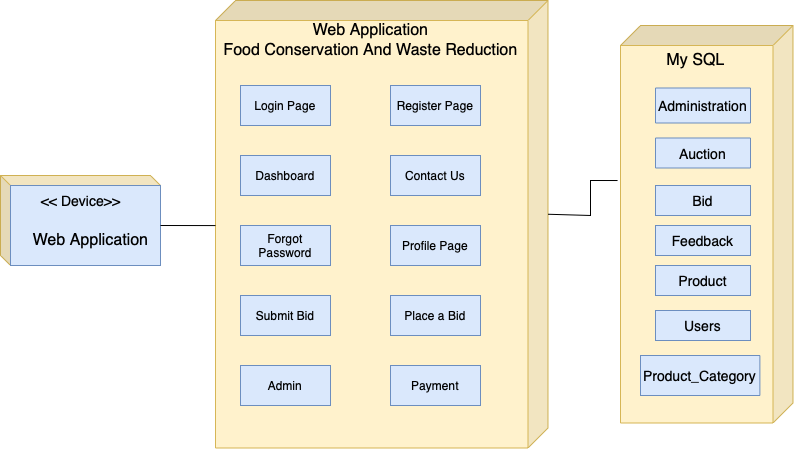
\includegraphics[width=15cm, height=15cm, keepaspectratio ]{projectReportTemplate/figures/Deployment Diagram.drawio.png}
    \caption{Deployment Diagram}
    \label{DD}
\end{figure}
\newpage
\section{Component Diagram}
The Component Diagram of our web application is shown in following Figure \ref{CD}. The component diagram helps in wiring the physical components in the system. The bidding, payment, contact us, managing users are all carried out thought the data base. and all of these are either done by users of the web application or admin.\\\\

\begin{figure}[!h]
    \centering
    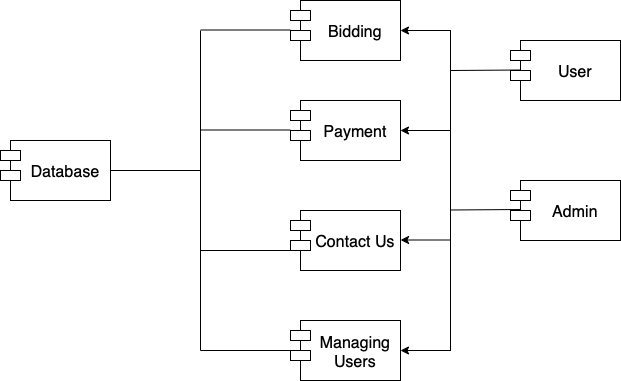
\includegraphics[width=15cm, height=15cm, keepaspectratio ]{projectReportTemplate/figures/Component Diagram.drawio.png}
    \caption{Component Diagram}
    \label{CD}
\end{figure}
